\section{Object 5}
\markright{Object 5}

\lipsum[5][1-4]

\begin{figure}[H]
	\centering

	\begin{subfigure}[b]{0.49\textwidth}
		\centering
		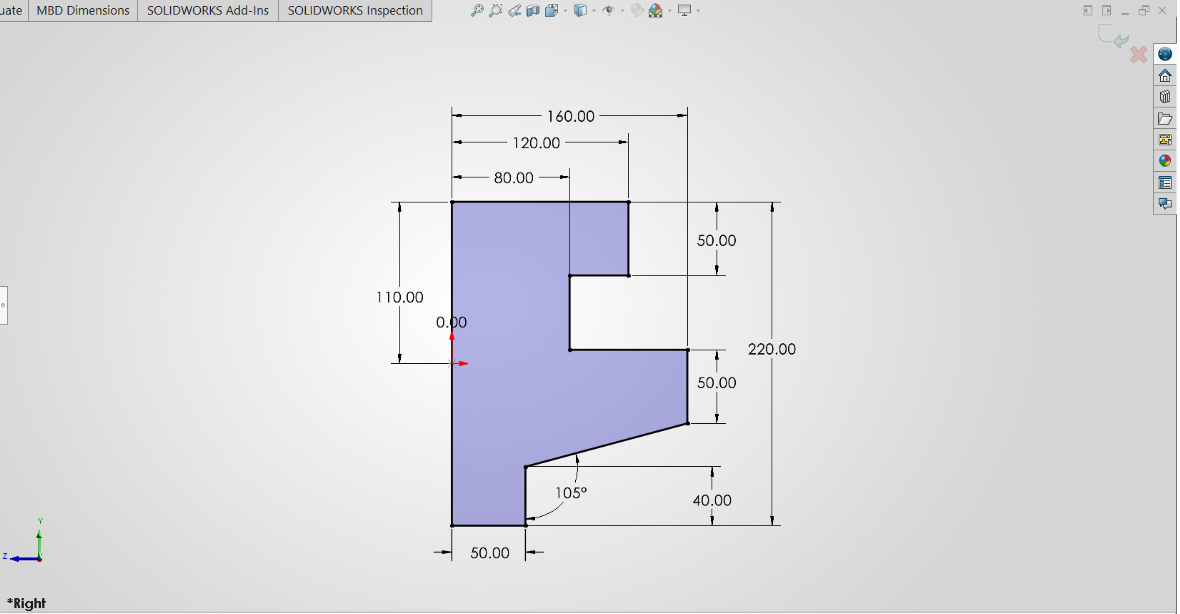
\includegraphics[width=\textwidth, keepaspectratio]{lab-01/assets/object-5/object-5-snap-1.png}
		\caption{2D drawing with dimentions}
	\end{subfigure}%
	\hfill
	\begin{subfigure}[b]{0.49\textwidth}
		\centering
		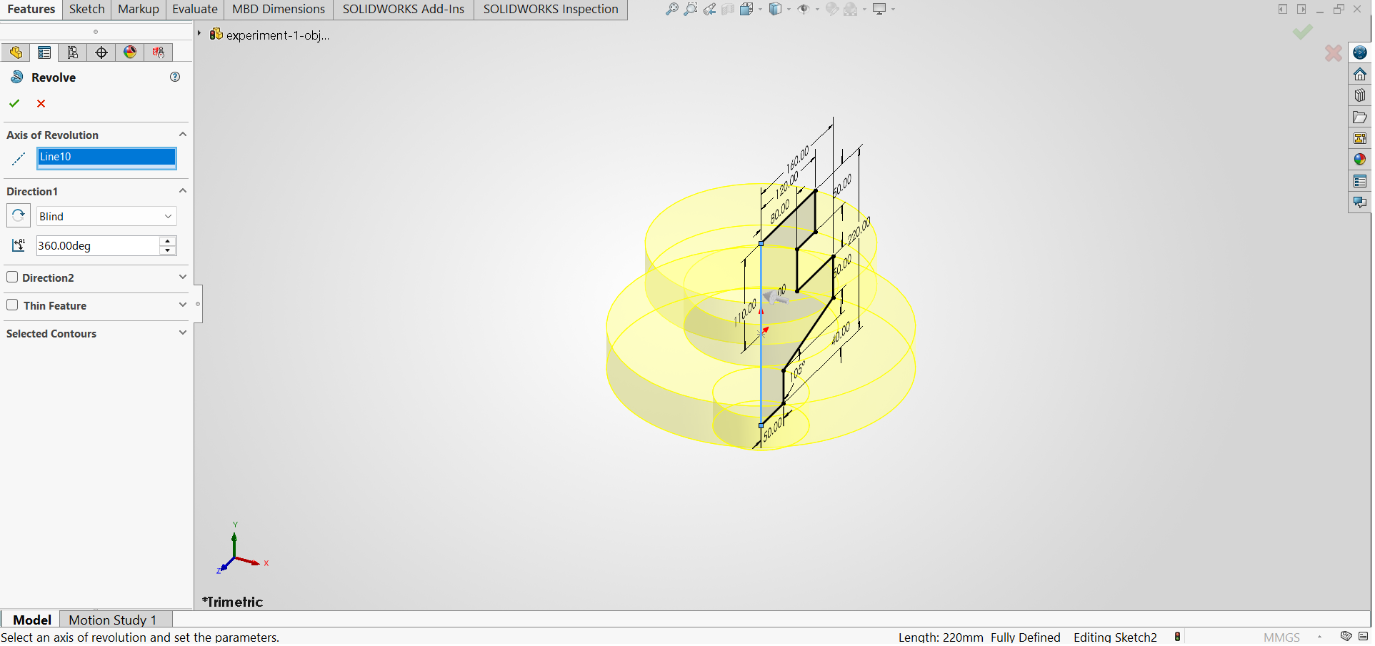
\includegraphics[width=\textwidth, keepaspectratio]{lab-01/assets/object-5/object-5-snap-2.png}
		\caption{Revolving around the vertical axis}
	\end{subfigure}%
	\vspace{0.5em}
	\begin{subfigure}[b]{\textwidth}
		\centering
		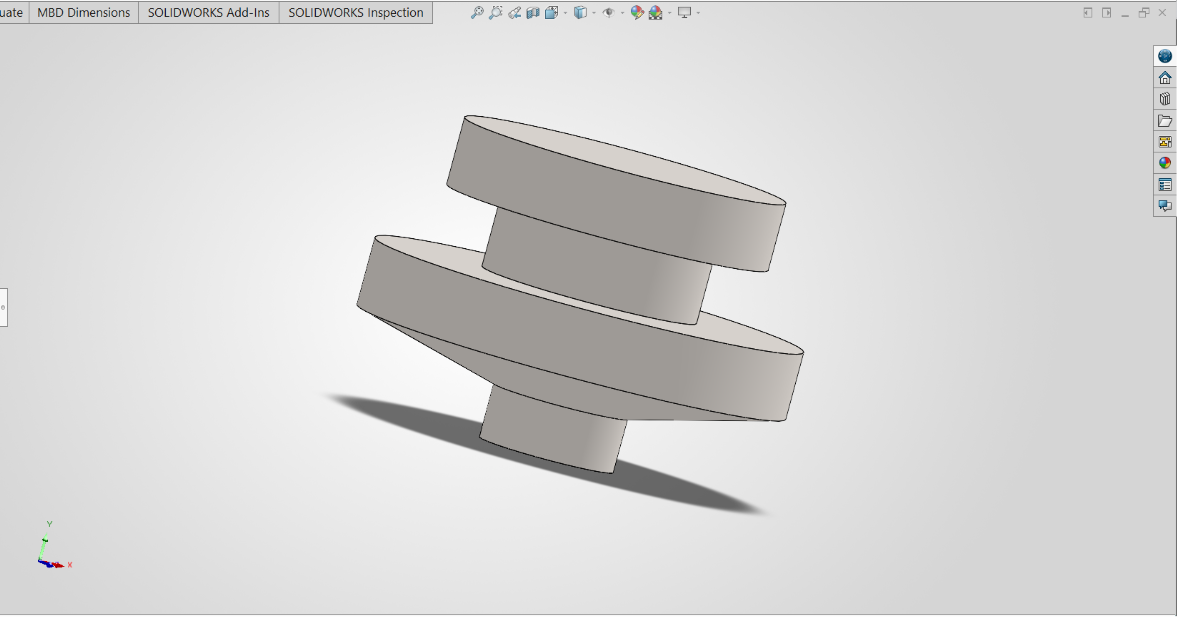
\includegraphics[width=\textwidth, keepaspectratio]{lab-01/assets/object-5/object-5-snap-3.png}
		\caption{Final Result}
	\end{subfigure}

	\caption{Snapshots while Designing Object 5 in Solidworks}
	\label{lab01_object_5}
\end{figure}

